\documentclass{article}
\usepackage{fullpage,proof,url,amssymb,amsmath,graphicx}


\newtheorem{theorem}{Theorem}
 
\def\barp{\bar{p}}
\def\HHB{{\mathrm{HHB}}}
\def\CS{\mathrm{CS}}
\def\calX{\mathcal{X}}
\def\bbR{\mathbb{R}}
\def\dx{\mathrm{d}x}
 
\newenvironment{proof}{\paragraph{Proof:}}{\hfill$\square$}
 
\newtheorem{fact}{Fact}
\newtheorem{lemma}{Lemma}
\newtheorem{definition}{Definition}

\begin{document}

\title{Thales circle theorem extended to Mahalanobis geometry}

\author{Frank Nielsen\\ {\tt Frank.Nielsen@acm.org}}
\date{\today}
\maketitle

 This column is also available in pdf: filename \url{MahalanobisThalesTheorem.pdf} 
\vskip 0.5cm


\section{Thales' theorem in Euclidean geometry}

In  planar Euclidean geometry, Thales' theorem  states that any triangle $pqr$  circumscribing a circle with one pair $(p,q)$ of antipodal points is necessarily 
a right triangle. 
A pair $(p,q)$ of antipodal points of a smooth convex object is such that the tangent lines at $p$ and $q$ are parallel to each other.
See Figure~\ref{fig:thales} for an illustration, and~\cite{Thales-2015} for a historical account (Thales of Miletus, 624--546 BC).

\begin{theorem}[Thales' circle theorem]
Any triangle circumscribed by a circle with one side being a diameter is right-angle.
\end{theorem}

\begin{figure}%
\centering
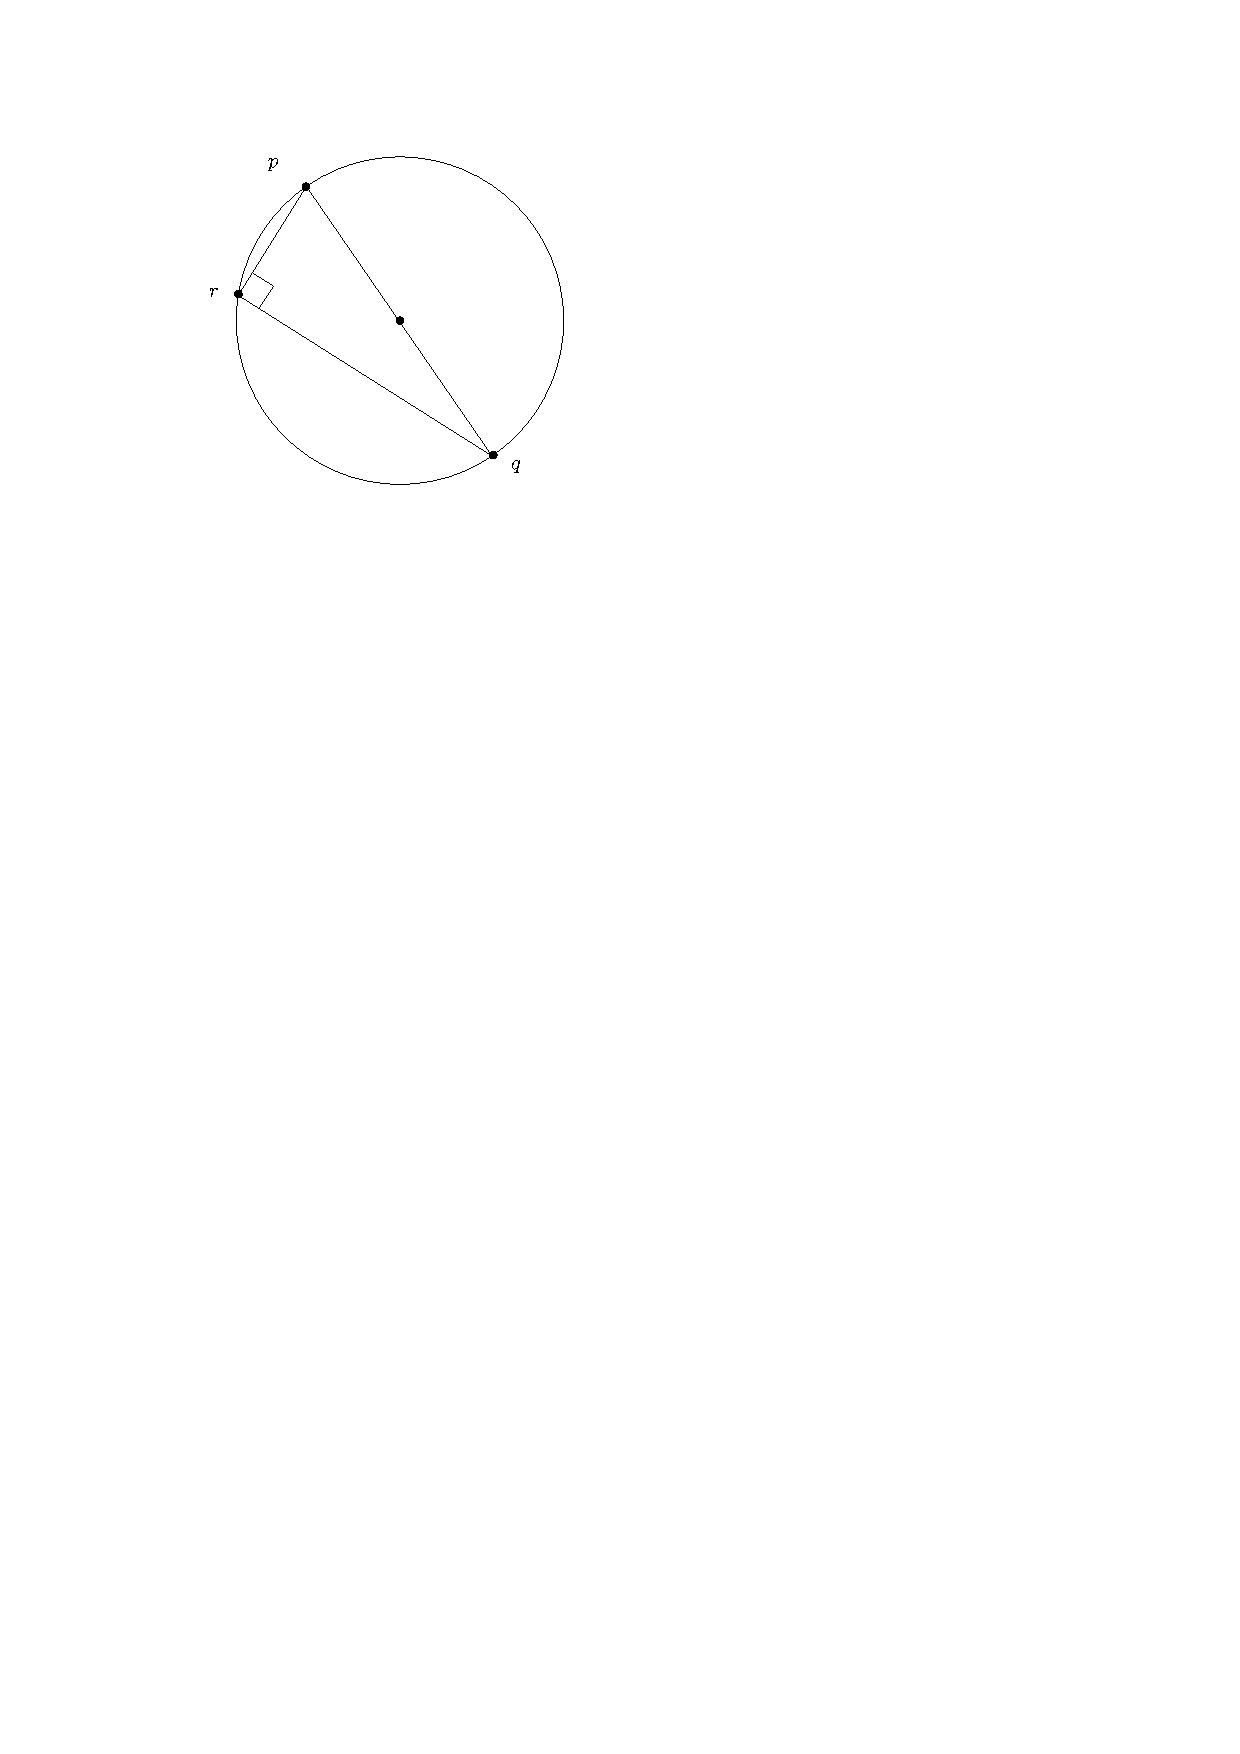
\includegraphics[width=0.3\columnwidth]{Fig-ThalesTheorem.pdf}%
\caption{Thales' circle theorem: Triangle $pqr$ is right-angle at $r$ where $[pq]$ is a diameter. $(p,q)$ is a pair of antipodal points.}%
\label{fig:thales}%
\end{figure}


\section{Thales' theorem in Mahanalobis geometry}

Let $D_A(p,q)$ denote the Mahalanobis distance between two points $p$ and $q$, for a positive definite matrix $A\succ 0$:
$$
D_A(p,q)=\sqrt{(p-q)^\top A (p-q)}=\|p-q\|_A.
$$
When $A=I$ is the $2\times 2$ identity matrix, the Mahalanobis distance amounts to the Euclidean distance $D_E(p,q)=\|p-q\|=\sqrt{(p-q)^\top  (p-q)}$.

A Mahalanobis circle~\cite{nielsen-2008} $C_A(c,r)$ of center $c$ and radius $r$ is defined as follows:
$$
C_A(c,r)=\{ x\ :\ D_A(c,x)=r\}.
$$
A Mahalanobis circle has an ellipsoid (Euclidean) shape.

Let us generalize Thales' theorem as follows:

\begin{theorem}[Thales' Mahalanobis circle theorem]
Any triangle circumscribed by a Mahalanobis circle with one pair of points being   antipodal  is right-angle.
\end{theorem}


\begin{proof}
Consider the Cholesky decomposition of $A$: $A=LL^\top=U^\top U$ with $L$ ($U=L^\top$) a lower triangular matrix (an upper triangular matrix, respectively) with positive diagonal elements.
The Mahalanobis distance amounts to calculate an ordinary Euclidean distance on affinely transformed points  $x'=L^\top x=U x$:
\begin{eqnarray*}
D_A(p,q) &=& \sqrt{(p-q)^\top LL^\top (p-q)},\\
 &=& D_E(L^\top p,L^\top q).
\end{eqnarray*}

Thus a Mahalanobis circles $C_A$ transforms affinely to a Euclidean circle $C_E=C_I$, and antipodal pairs of points on $C_A$ 
remain antipodal in $C_E$.

Two vectors $u$ and $v$ are perpendicular in the Mahalanobis geometry  if and only if $u^\top A v=0$.
That is, if $u^\top A v= u^\top LL^\top v= (L^\top u)^\top L^\top v={u'}^\top v'=0$.
 
A triangle $pqr$ circumscribing the Mahalanobis circle $C_A$ with $(p,q)$ an antipodal pair in Mahalanobis geometry transforms into a
triangle $p'q'r'$ circumscribing the Euclidean circle $C'=\{L^\top x\ :\ x\in C_A(c,r) \}$ with $(p',q')$ an antipodal pair.
Therefore $p'q'r'$ is a right-angle triangle in Euclidean geometry, and:

\begin{eqnarray}
(q'-r')^\top (p'-r') &=& 0,\\
(L^\top(q-r))^\top L^\top (p-r) &=& 0,\\
(q-r)^\top L L^\top (p-r) &=&0,\\
(q-r) A (p-r) &=& 0.
\end{eqnarray}
Therefore, $pqr$ is a right-angle triangle in Mahalanobis geometry.
\end{proof}


\begin{figure}%
\centering
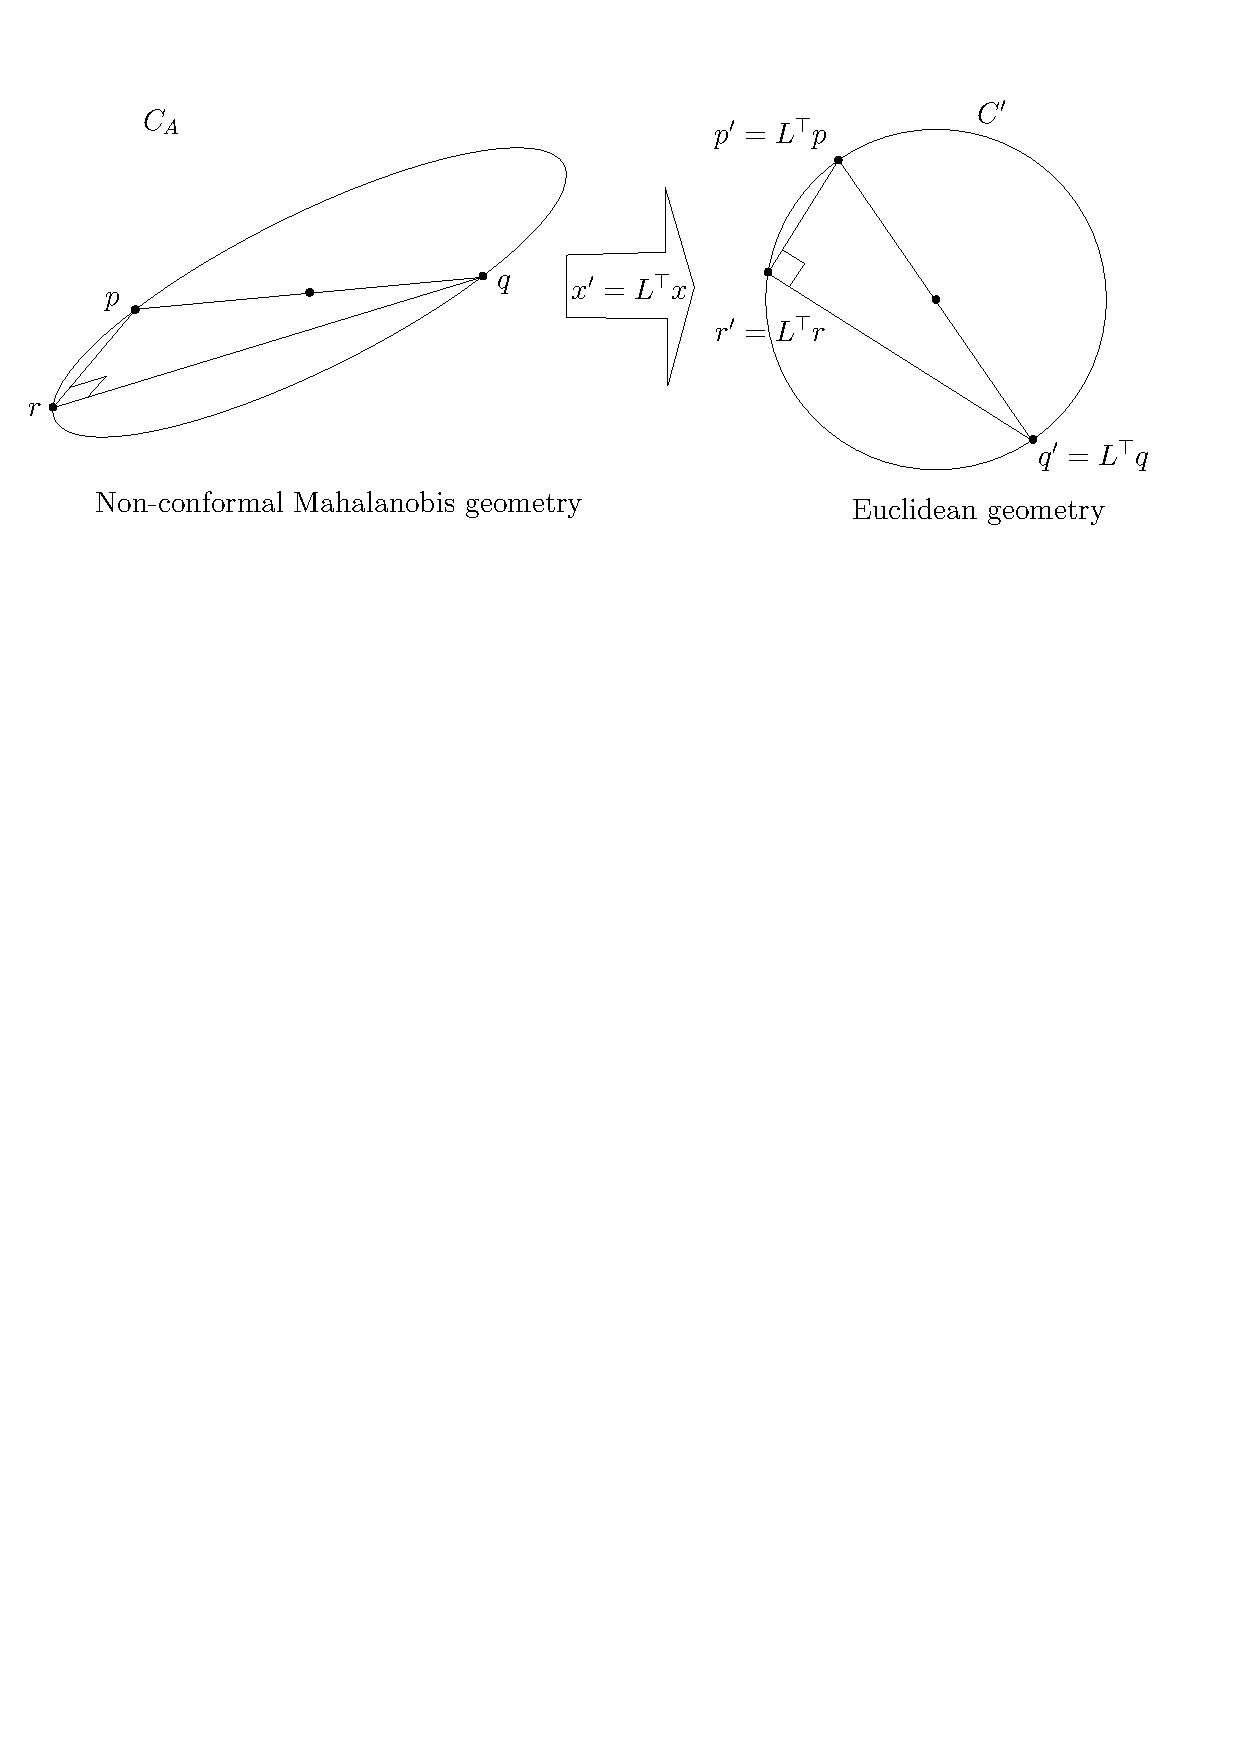
\includegraphics[width=0.7\columnwidth]{Fig-ThalesMahalanobisTheorem.pdf}%
\caption{Thales' circle theorem in Mahalanobis geometry: Triangle $pqr$ is right-angle at $r$ where $[pq]$ is an antipodal pair of points.
Notice that Mahalanobis geometry is generally not conformal so that a Mahalanobis right-angle does not visualize as a Euclidean right-angle.}%
\label{fig:mahthales}%
\end{figure}


Note that Mahalanobis geometry is not conformal when $A\not =\lambda I$ (for $\lambda>0$), the scaled identity matrix.
Therefore angles are not preserved in Mahalanobis geometry: 
That is, a Mahalanobis right-angle cannot be visualized as a Euclidean right-angle in general.


Squared Mahalanobis distances are the only symmetric Bregman divergences~\cite{BVD-2010}.
But Thales' theorem do not extend to other (asymmetric) Bregman divergences.





\bibliographystyle{plain}
\bibliography{MahalanobisThalesTheoremBIB}
\end{document}